%% Преамбула TeX-файла

% 1. Стиль и язык
\documentclass[utf8x, usepscyr]{G7-32} % Стиль (по умолчанию будет 14pt)

% Остальные стандартные настройки убраны в preamble.inc.tex.
\sloppy

% Настройки стиля ГОСТ 7-32
% Для начала определяем, хотим мы или нет, чтобы рисунки и таблицы нумеровались в пределах раздела, или нам нужна сквозная нумерация.
\EqInChapter % формулы будут нумероваться в пределах раздела
\TableInChapter % таблицы будут нумероваться в пределах раздела
\PicInChapter % рисунки будут нумероваться в пределах раздела

% Добавляем гипертекстовое оглавление в PDF
\usepackage[
bookmarks=true, colorlinks=true, unicode=true,
urlcolor=black,linkcolor=black, anchorcolor=black,
citecolor=black, menucolor=black, filecolor=black,
]{hyperref}

% Изменение начертания шрифта --- после чего выглядит таймсоподобно.
% apt-get install scalable-cyrfonts-tex

\IfFileExists{cyrtimes.sty}
    {
        \usepackage{cyrtimespatched}
    }
    {
        % А если Times нету, то будет CM...
    }

\usepackage{graphicx}   % Пакет для включения рисунков
\DeclareGraphicsExtensions{.jpg,.pdf,.png}
% С такими оно полями оно работает по-умолчанию:
% \RequirePackage[left=20mm,right=10mm,top=20mm,bottom=20mm,headsep=0pt]{geometry}
% Если вас тошнит от поля в 10мм --- увеличивайте до 20-ти, ну и про переплёт не забывайте:
\geometry{right=20mm}
\geometry{left=30mm}



% Произвольная нумерация списков.
\usepackage{enumerate}

\setcounter{tocdepth}{4} %Подробность оглавления
%4 это chapter, section, subsection, subsubsection и paragraph
%3 это chapter, section, subsection и subsubsection
%2 это chapter, section, и subsection
%1 это chapter и section
%0 это chapter.

\usepackage{comment}

\usepackage{algorithm}
\usepackage{algpseudocode}
\usepackage{listings}
\usepackage{color}



\lstset{frame=tb,
	language=Java,
	aboveskip=3mm,
	belowskip=3mm,
	showstringspaces=false,
	columns=flexible,
	basicstyle={\small\ttfamily},
	numbers=none,
	numberstyle=\tiny\color{gray},
	keywordstyle=\color{blue},
	commentstyle=\color{dkgreen},
	stringstyle=\color{mauve},
	breaklines=true,
	breakatwhitespace=true,
	tabsize=3,
	language=Java
}

\definecolor{dkgreen}{rgb}{0,0.6,0}
\definecolor{gray}{rgb}{0.5,0.5,0.5}
\definecolor{mauve}{rgb}{0.58,0,0.82}
\usepackage{pscyr}

\renewcommand{\rmdefault}{ftm}

\begin{document}


\frontmatter % выключает нумерацию ВСЕГО; здесь начинаются ненумерованные главы: реферат, введение, глоссарий, сокращения и прочее.
\begin{center} 

\large Казанский (Приволжский) Федеральный Университет \\ Высшая Школа Информационных Технологий и Интеллектуальных Систем\\[5.5cm] 

\huge Выпускная квалификационная работа\\[0.6cm] % название работы, затем отступ 0,6см
\large РАЗРАБОТКА ИНСТРУМЕНТА АВТОМАТИЗАЦИИ ДЕЙСТВИЙ ДЛЯ ИГРОВОГО ДВИЖКА UNITY \\[3.7cm]


\end{center} 

\begin{flushright}
Выполнил: студент гр. 11-605 \\
О.А. Бедрин \\
\end{flushright}


\vfill 

\begin{center} 
\large Казань 2020
\end{center} 

\thispagestyle{empty}

\thispagestyle{empty}
\setcounter{page}{0}
\tableofcontents
\clearpage


\Introduction
\section*{Постановка проблемы}
В жизненном цикле разработки каждого программного обеспечения (ПО) присутствует этап приемо-сдаточных работ. Перед тем как передавать ответственному за этот этап уставному органу проекта собранное ПО, необходимо провести один из завершающих этапов разработки, а именно регрессионное тестирование. Алгоритм проведения данного вида тестирования технически довольно прост: создаются сценарии пользовательского поведения в виде диаграммы вариантов использования, выбирается формальный исполнитель, который шаг за шагом выполняет действия описанные в главных, а затем альтернативных потоках вариантов использования.

Вопрос выбора формального исполнителя здесь стоит довольно остро, так как это напрямую влияет на стоимость разработки. Для разных групп используемых технологий разработки данная проблема решается по-разному. Например, для популярных платформ, таких как PC, Web, iOS, Android, уже существуют разные автоматические формальные исполнители для приложений с различными возможностями и характеристиками, для однократной записи и множественного проигрывания действий потоков. Ими, например, являются Selenium, Appium, Robotium и UI Automator. Формы решения вопроса выбора исполнителя существуют разные, например, для Web используется WebDriver для записи и имитации ввода \cite{selenium}, для iOS и Android используется система RPC вызовов \cite{rpc_testing}, если же нет возможности вмешаться в поток ввода для облегчения записи, то используется компьютерное зрение для распознавания того, как и с чем взаимодействует пользователь \cite{appium_opencv}. Метод зачастую довольной эффективный для графических систем с конечным набором однотипных элементов (напр. Класс систем Windows, Icons, Menus, Pointers (WIMP) \cite{wimp}), однако гораздо менее точный при большом разнообразии динамических графических элементов. В дополнение вышеописанные исполнители для данных платформ ограничены устройствами ввода, а именно клавиатурой и мышкой.

Особняком здесь стоит задача о выборе формального исполнителя для тестирования игровых приложений на популярной платформе для разработки приложений визуализации и игр \textit{Unity} \cite{habr}. Каждая из вышеупомянутых форм решения вопроса в этом случае проигрывает и в эффективности, и в степени удобства интеграции инструмента записи и проигрывания действий, так как зачастую игры насыщены динамическими графическими элементами, а некоторые игры вообще не имеют графический интерфейс. В отличие от других платформ, \textit{Unity} -- не ограничена устройствами ввода. Поэтому часто формальным исполнителем здесь становится группа специалистов или других людей которые играют роль тестировщиков. Им, частично или полностью, выдаётся информация о действиях внутри потоков и они их исполняют, составляя в заключении необходимые отчёты. В данном случае стоимость разработки также повышается ввиду создания и поддержки системы контроля работы тестировщиков.

Альтернативный подход к регрессионному тестированию на платформе \textit{Unity} является автоматизированное модульное тестирование. Однако, при использовании данного подхода необходимо для каждого основного потока писать комплекс из юнит-тестов (алгоритмов тестирования описанных в коде ПО и исполняемых в контексте с ним средствами выбранной платформы). Время написания подобного комплекса примерно равно объёму времени этапа основной разработки при этом появляется необходимость поддержки в дополнении к основной кодовой базе ещё и юнит-тестов со всеми вытекающими издержками.

\section*{Цель и задачи разработки}
Целью данной работы является реализация и применение формы решения описанной выше проблемы регрессионного тестирования для игровых приложений платформы \textit{Unity} в виде импортируемой группы ассетов (исходных файлов кода и пред заготовленных графических и модульных инструментов). 

Реализуемое решение основано на вышеописанных подходах для платформ PC, Web и др., и на возможности декорирования методов взятия ввода, обусловленной внутренней архитектурой платформы. Две главных особенностей данного решения -- это высокая точность распознавания и перехвата ввода и возможность избежать регулярных потерь времени при человеческом тестировании за счёт однократной записи ввода не только с клавиатуры и компьютерной мыши, но и любого другого периферийного устройства и дальнейшего проигрыша записанного ввода по необходимости регрессионного тестирования.

В настоящей выпускной квалификационной работе рассматриваются задачи связанные напрямую с исследованием применения инструментария взятия ввода, а также задачи цикла разработки данных ассетов на платформе \textit{Unity}.

В первой главе рассматриваются исследование среднего количества использований внутреннего инструмента взятия ввода платформы \textit{Unity} среди самых значимых и популярных проектов на данной платформе. Происходит анализ класса совместимых приложений с описанными в данной работе ассетами, а также определение теоретической базы приёмов программной инженерии, которые были использованы в рамках данной работы.

Во второй главе описан процесс разработки описываемой группы ассетов, состоящий из трёх подпроцессов: реализация вспомогательных систем для статистических исследований и управления зависимостями, создание базовой системы интеграции ассетов и реализация основных систем, позволяющих осуществить запись и проигрывание, хранение, загрузку, экспорт и импорт действий.

Дополнительная задача при разработке данной группы ассетов описанная в конце второй главы -- возможность сериализовывать, экспортировать и импортировать записанные данные для последующего использования. Например для построения сценария для тренажеров в виртуальной реальности \cite{disser} или для генерации сценария обучающего тренажера \cite{vr-simulators}, что поможет избежать рутинной работы по формированию треков обучения \cite{visual-editor}.

Третья глава посвящена циклу разработки окон управления группой ассетов после интеграции в сторонний проект, а также разработке и развёртыванию онлайн-документации, в которой описывается процесс использования окон управления. Здесь же описываются принципы дополнения и расширения исходной кодовой базы описываемых ассетов для всех желающих сторонних разработчиков.

Четвертая и заключительная глава рассматривает опыт портирования и применения разработанной группы ассетов внутри проекта виртуальной био-технологической лаборатории.

\section*{Объект и предмет разработки}
Объектом разработки является процесс автоматизации регрессионного тестирования для приложений с богатой или отсутствующей динамической графикой и пользовательским интерфейсом на платформе \textit{Unity}. В качестве предмета разработки в данной работе описывается группа ассетов предназначенных для автоматизации действий пользователя.

Иными словами, результатом представлен набор дополнительных окон и утилит для редактора \textit{Unity} для записи и проигрывания сценариев, автоматической интеграции группы ассетов в готовую кодовую базу стороннего проекта, а также для сохранения и загрузки записанных сценариев представляющих собой входные данные со всех периферийных устройств, что были активны во время работы приложения, в которое группа ассетов была импортирована.

Дополнением к результату является документация к пользованию разработанными ассетами, их расширению для нужд сторонних разработчиков, а также видеофайл, демонстрирующий работу с симулятором VR устройства в проекте DML BioLab \cite{biolab}, где происходит запись и проигрывание первого пункта первого сценария.


\mainmatter

\chapter{Проектирование}
\label{cha:ch_1}

\subsection{Класс совместимых приложений}
Описанный в данной работе набор ассетов Automated Test Framework (ATF) предназначен для автоматизации действий с целью функционального тестирования. Его можно интегрировать c любым  \textit{Unity}-проектом, система ввода которого построена вокруг класса из стандартной библиотеки \textit{Unity} по взаимодействию с вводом Input. Под это описание подходит большая часть \textit{Unity}-приложений и в этом выражена универсальность предложенного решения. Ранее среди свободных для использования ассетов не было представлено решений для автоматизации ни success-тестов, ни тестирования главного потока сценария использования (use-case), ни других подходов для функционального тестирования приложений, кроме как через механизмы стандартного пакета unit-тестирования \textit{Unity}. Однако как бы ни был хорош подход использования инструментария unit-тестирования, для того чтобы покрыть все возможные сценарии действий внутри проекта, пришлось бы либо писать свой модуль тестов под каждый из аспектов, либо же на его основе реализовывать сложную универсальную систему.

\subsection{Определение теоретической базы}
\begin{figure}[H]
	\centering
	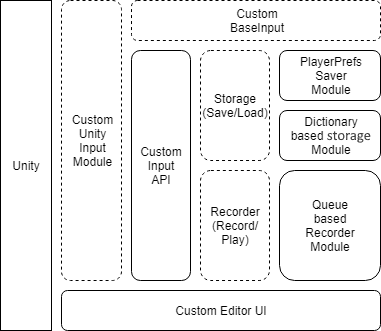
\includegraphics[width=\linewidth]{platform.png}
	\caption{Диаграмма платформы решения}
	\label{platform}
\end{figure}

На этапе проектирования была составлена диаграмма платформы (см. рис. \ref{platform}), каждый блок которой -- это изолированная группа методов API, решающая свои задачи: 
\begin{itemize}
	\item \textit{Unity} -- непосредственно сам игровой движок;
	\item \textit{Custom Unity Input Module} -- абстракция, объединяющая управление вводом;
	\item \textit{Custom Input API} -- собственно API, который вызывает нативные методы по запросу ввода;
	\item \textit{Custom BaseInput} --  сущность, которяа является реализацией объекта обработки потока данных через мост (Bridge), объединяя статичные методы по перехвату/симуляции ввода и обернутые события (Events);
	\item \textit{Storage} --  абстракция, отвечающая за функционал хранения и манипуляции записанных действий;
	\item \textit{Recorder} -- абстракция, отвечающая за запись действий;
	\item \textit{Custom Editor UI} -- система пользовательских окон для управления всеми процессами;
	\item \textit{PlayerPrefs Save/Load Module} -- система реализации абстракции модуля по сохранению/загрузке записанных действий на базе стандартного класса PlayerPrefs;
	\item \textit{Dictionary based Module} -- реализация абстракции хранилища записанных действий, основанная на структуре данных ``Словарь'';
	\item \textit{Queue based Recorder Module} -- реализация абстракции, отвечающей за запись действий, основанная на структуре данных ``Очередь''.
\end{itemize}

Для выполнения поставленных задач было разработано решение, являющееся, по своей сути, модифицированным адаптером, который перехватывает и симулирует ввод. Для его эффективной реализации стало органичным использовать несколько архитектурных паттернов:
\begin{itemize}
	\item
	\textit{Interceptor} -- шаблон для перехвата и подмены входных данных с периферийных устройств \cite{interceptor};
	\item
	\textit{Broker} -- шаблон для интеграции и взаимодействия с встроенной системой управления входными данными \textit{Unity} \cite{broker};
	\item
	\textit{PAC (Presentation–abstraction–control)} -- шаблон для организации взаимодействия зависимых систем \cite{pac}.
\end{itemize}

Для подмены стандартного класса Input был создан перехватчик ATFInput (см. рис. \ref{atfInput}), который наследуется от стандартного класса BaseInput для использования встроенной пользовательской системы управления вводом. ATF -- это сокращение от английского Automated Test Framework, которое переводиться как: фреймворк автоматизированного тестирования. Так как класс Input содержит в себе только статичные методы, декорация их для перехвата внутри ATFInput позволила совместить и классический перехват ввода и облегчить в дальнейшем перехват событий ввода. Иначе говоря, было проведено совмещение перехватчика для класса Input и класса BaseInput  для взаимодействия с событиями ввода внутри \textit{Unity}. 

\begin{figure}[H]
	\centering
	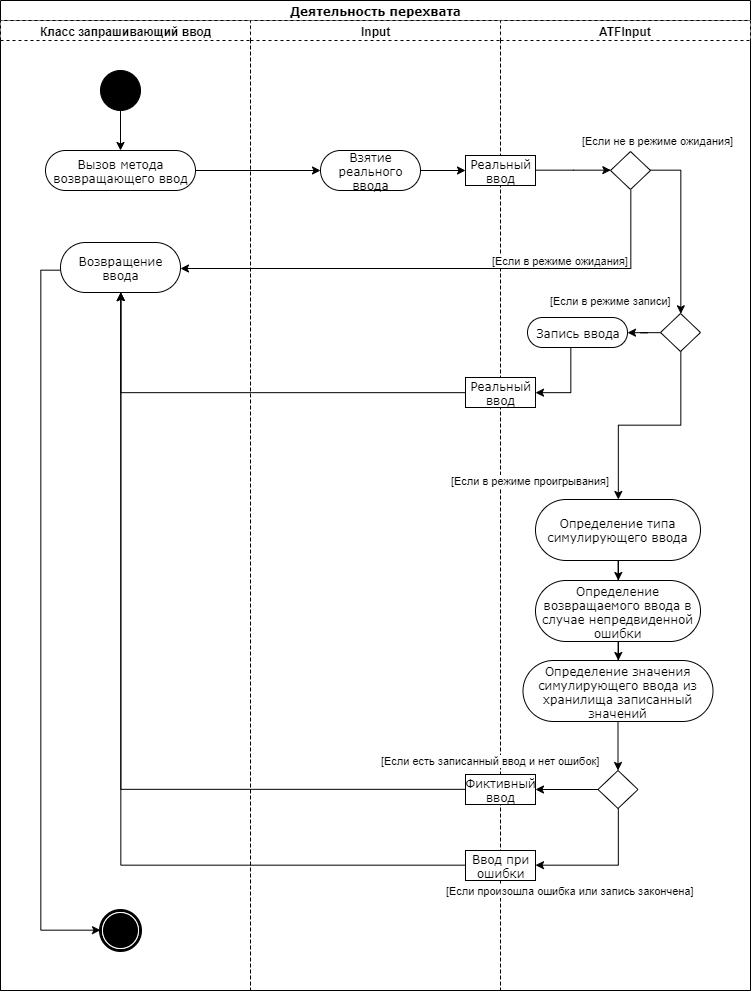
\includegraphics[width=\linewidth]{atfInput.png}
	\caption{Диаграмма деятельности ATFInput}
	\label{atfInput}
\end{figure}


Для интерпретации (проигрывания) первоначально использовался паттерн Interpreter с терминалами ожидания внутри Coroutine. Однако после попытки тестовой реализации данного шаблона был произведен отказ от этого шаблона в пользу метода записи, основанного на структуре данных ``Очередь'', так как для правильной работы терминалов ожидания необходимо было просчитывать заранее действия пользователя, что затруднительно.
\chapter{Внутренние модули и системы группы ассетов}
\label{cha:ch_2}

Процесс разработки внутренних модулей и систем в данной главе представлен в виде краткого описания главных аспектов модуля или системы, которое дополненно листингом с подробной иллюстрацией бизнес-процесса.

\section{Вспомогательные системы}
Все вспомогательные системы, кроме spider-программы описанной ниже, спроектированы по паттерну ``Одиночка'' (Singleton) для \textit{Unity}, что означает, что на сцене и в ссылках на экземпляры класса компонента будет находиться только одна инициализированная на сцене сущность.

\subsection{Spider-программа для сбора данных с GitHub.com}
Для сбора данных и проведения эксперимента по вычислению бутстраповского доверительного интервала в рамках данной работы была разработана программа позволяющая перемещаться по страницам сайта GitHub.com с возможностью сбора необходимых данных. Данная программа имеет префикс spider, так как она подобно пауку может ползать во всемирной паутине улавливая данные.

\subsubsection*{Инструментарий для проектирования spider-программы}
В качестве основы для spider-программы использовался фреймворк Scrapy \cite{scrapy}. Данный фреймворк автоматизирует решение задач о том какими именно инструментами и каким образом происходит получение веб-страниц. На вход ему задаётся массив из необходимых URL адресов, а также функция по обработке данных полученных по ним веб-страниц. Его использование позволило сконцентрироваться на алгоритме обработки данных, что дало избежать написания сквозного кода (усложняющего чтение кода).

\subsubsection*{Алгоритм поведения spider-программы}
На вход алгоритма по обработки данных (см. листинг \ref{spider}) подается один из адресов поиска по сайту с настроенным фильтром: самый релевантный запросу, самый популярный по рейтингу звёзд, с самым большим количеством форков и самые стабильно обновляющийся проект (где средний разброс времени между коммитами у проекта невелик). Далее происходит вычленение по страницам полные названия репозиториев, которые используются для выгрузки всех доступных файлов исходного кода репозитория по очереди. Выгруженные файлы исходного кода затем фильтруются по ключевому слов \textit{Input}, что превращает поток файлов в поток сниппетов кода (блоков кода) с использованием слова Input в той или иной команде или функции. На выходе данный поток ещё более фильтруется, но уже по регулярному выражению, которое выявляет любые использования класса Input. Затем вычисляется размер результирующего потока, который впоследствии попадает в выборку рядом с полным именем просмотренного репозитория.

\subsubsection*{Формат выходных данных spider-программы}
В качестве результата работы этапа сборки данных, в корневую папку spider-программы сохраняется .csv файл со структурой идентичной таблице \ref{tab:sample}.

\subsubsection*{Утилиты spider-программы для проведения расчётов}
В дополнении к ядру spider-программы были реализованы вспомогательные утилиты для сбора данных в один .csv файл (см. листинг \ref{form_main_data}) и для проведения бутстрапа и расчётов (см. листинг \ref{bootstrap_experiment}). Стоит заметить, что проведение бутстрапа и расчётов задача вычислительно ёмкая, поэтому предложенный алгоритм автоматически использует все доступные ядра на процессоре, чтобы провести вычисления параллельно. 

В итоге, на выходе работы spider-программы создаётся диаграмма рассеяния с шестиугольным фильтром указывающая на нижнюю и верхнюю границы доверительного интервала среднего (см. рис. \ref{experiment}).

\subsection{Синглтон для объектов сцены}
Подробное описание основного функционала данного шаблона представлено в листинге \ref{monoSingleton}. Если описывать в двух словах реализацию этого довольно простого паттерна, то поведение наследников данного класса сводится к тому, что если при вызове поля Instance на сцене не окажется уже установленного объекта, то он создается и конфигурируется автоматически.

\begin{figure}[h]
	\centering
	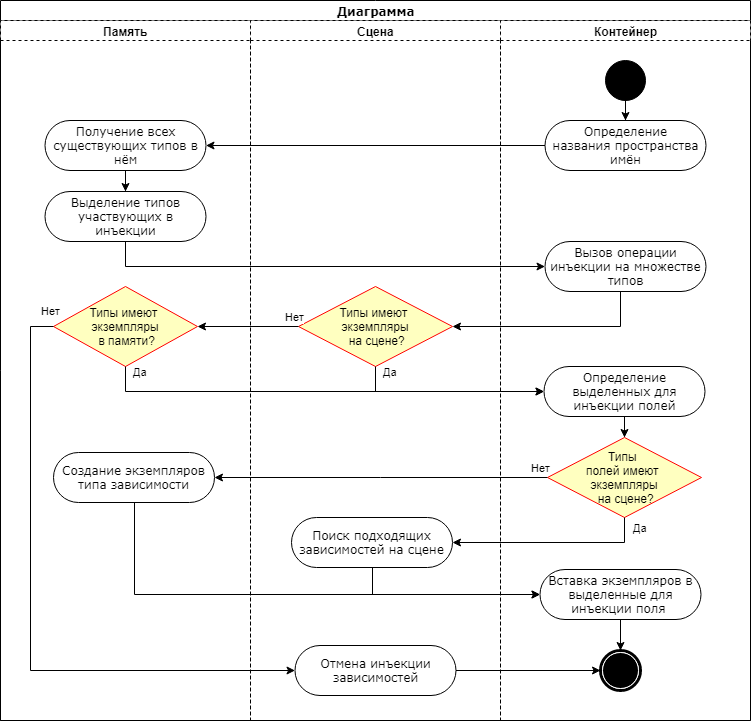
\includegraphics[width=\linewidth]{containerDI.png}
	\caption{Диаграмма деятельности работы DI контейнера для \textit{Unity}}
	\label{injectionIllustration}
\end{figure}

\subsection{DI контейнер для объектов сцены}
В качестве основного функционала контейнера представлен метод, который осуществляет проверку на участие в инъекции зависимостей, поиск подходящей зависимости и непосредственно инъекцию. Все три этапа работают по известному механизму описанному в стандарте JSR-299 \cite{jsr}, а именно: с помощью атрибутов, которые выполняют роль аннотаций, помечаются классы, участвующие в инъекции и поля, в которые нужно её проводить, далее контейнер на этапе запуска проекта проводит все инъекции. Бизнес-логика данного метода подробно представлена в листинге \ref{injectType}.

Для того чтобы провести инъекцию в целом продукте, также был реализован механизм, который вызывает вышеупомянутый метод на каждом найденном по названию пространства имен типе. Инъекция происходит в двух случаях: объекта из сцены в объект на сцене и объекта из памяти в объект на сцене. 

Данный принцип сюръекции нужен только для того, чтобы предупреждать появления ошибок при использовании или дополнении данного контейнера, когда объект, куда происходит инъекция, не создан на сцене или не инициализирован в памяти. Работа контейнера кратко описана в диаграмме деятельности на рис. \ref{injectionIllustration}.

\section{Модули инициализации и перехвата ввода}
Для того чтобы сократить количество лишних действий после импортирования данной группы ассетов в сторонний проект, был реализован модуль инициализации, главная цель которого заключалась в автоматической настройке основных систем при переходе в Play Mode.

Модуль перехвата является ядром разрабатываемой группы ассетов, в основе которого лежит тот факт, что если полностью скопировать сигнатуры статических методов стандартного класса Input, то для дальнейшей интеграции и использования необходимо будет лишь использовать имя другого класса, вместо имени Input. Все же основные аспекты стандартного взятия ввода останутся нетронутыми.

\subsection{Базовый инициализатор}
Для легкой интеграции данного продукта был реализован префаб пустого экземпляра класса GameObject, композиция которого содержит в себе единственный компонент (см. листинг \ref{initializer}) -- его работа  иллюстрируется алгоритмом \ref{alg:initializer}.

Механизм работы заключается в следующем: каждая из систем наследуется от интерфейса, который используется в зависимых классах и куда происходит инъекция. Сделано это было с требованием последнего принципа SOLID. Данный интерфейс также наследуется от другого интерфейса IATFInitializable, который содержит в себе единственный метод, отвечающий за инициализацию всех параметров системы после её создания на сцене путем вызова поля Instance. Далее происходит инициализация DI контейнера, настройка его на инъекцию в пространство имён ATF и вызов самой инъекции.

\subsection{Расширенный инициализатор}
Чтобы избежать дополнительного вмешательства в исходный код реализации базового инициализатора при добавлении новых систем, был создан механизм составления очереди на вызов поля Instance и инициализацию путём маркировки новых систем атрибутом AtfSystem. Другими словами, чтобы добавить новую систему при этом не вмешиваясь в код базового инициализатора, необходимо чтобы добавляемая система типа T наследовалась от класса MonoSingleton<T> и при этом её класс был бы помечен соответствующим атрибутом.

\subsection{Адаптер для класса Input}
Далее представлен алгоритм \ref{alg:input}, составляющий бизнес-процесс класса адаптера, в котором и осуществляется перехват и вычисление относительно текущего состояния систем управления записью и хранилища (см. листинг \ref{input}). Кратко описывая принцип работы, можно выделить три ключевых метода: $Intercept, GetCurrentFakeInput, RealOrFakeInputOrRecord$. Они вызываются стеком, начиная с первого метода. 

Первым делом осуществляется перехват (в данном примере) входных данных Input.anyKeyDown, затем происходит вычисление записанного результата из STORAGE с помощью метода $GetCurrentFakeInput$, независимо от того, записывается ли процесс или проигрывается. Далее происходит решение, что выдавать на выход функции anyKeyDown в зависимости от того, в каком сейчас состоянии проигрыватель. Если происходит проигрывание, то выдается результат, который был сохранен в хранилище, если же происходит запись, то выдается результат Input.anyKeyDown и он же записывается в хранилище, а если ничего не происходит, то просто выдается результат, как если бы прослойки для записи вообще не существовало.

\subsection{Расширенный модуль ввода}
Этот пользовательский модуль (см. листинг \ref{inputModule}) был спроектирован с целью дальнейшего расширения функционала по перехвату на внутреннюю систему обмена сообщениями внутри \textit{Unity}. Можно заметить, где конкретно реализован шаблон проектирования Bridge -- внутри StandaloneInputModule уже созданы события и описания поведения для работы с сообщениями ввода с периферийных устройств. Именно эти события и будут в будущем подвержены перехвату.

\section{Основные системы группы ассетов}
Далее под словом ``система'' будет пониматься класс типа T который наследуется от класса MonoSingleton<T> и обладает однородным интерфейсом с другими ``системами''.

\subsection{Система записи и проигрывания}
За основу системы записи и проигрывания был взят интерфейс (cм. листинг \ref{iRecorder}), регламентирующий поведение, схожее с недетерминированным автоматом, структура которого напоминает полный граф. Дело в том, что данная система подразумевает, что может происходить запись только одной структуры, которая составляет из себя набор различных вводов, в одну единицу вызова.

То есть, для того чтобы начать запись, необходимо первым делом использовать статичные методы ATFInput, во-вторых вызвать метод SetCurrentRecordingName и далее уже вызвать один из методов, изменяющих состояние проигрывателя, в данном конкретном случае -- StartRecord. Реализация интерфейса основана на главном свойстве структуры данных ``Очередь'' -- когда происходит запись, то пара FakeInput и объект значения записывается в очередь которая распологается внутри системы хранилища. Там же, при проигрывании выполняется выгрузка данной очереди в отдельную переменную и при каждом вызове перехватываемого метода, просто происходит выдача того, что было первым в этой очереди и так, раз за разом, пока вся очередь не опустошится.

\subsection{Система хранилища действий}
За основу поведения системы хранилища действий был взят интерфейс IATFActionStorage (см. листинг \ref{iStorage}), регламентирующий поведение книжной полки (статичного хранилища данных).

Принцип работы довольно прост, реализация данного хранилища базируется на вложенной структуре данных ``Словарь'' или иногда его называют хеш-таблицей. Внутри системы находятся поля следующих типов:
\begin{itemize}
	\item 
	\begin{verbatim}
	Dictionary<string, Dictionary<FakeInput, 
		Dictionary<object, Queue<Action>>>>;
	\end{verbatim}
	\item 
	\begin{verbatim}
	Dictionary<FakeInput, Dictionary<object, 
		Queue<Action>>>.
	\end{verbatim}
\end{itemize}

Первый тип -- это основное хранилище, туда происходит загрузка свежезаписанных сценариев, а также из жесткой памяти, например, из реестра. Второй тип -- это та самая переменная, в которую копируется очередь определенного типа ввода и которая опустошается на протяжении каждого перехватываемого вызова проверки ввода. Другие же методы отвечают за операции управления над самим хранилищем.

\subsection{Решение проблемы избыточности хранилища действий}
При использовании в основе хранилища стандартной структуры данных ``Очередь'' для хранения записываемых действий было замечено, что при каждом использовании функции записи очередного действия, создаётся новый объект параметра ввода и записывается в очередь. Такой подход приводит к чрезвычайно большим очередям наполненным одинаковыми действиями. Использование класса Input возможно только в рамках главного цикла компонента, итерации которого вызываются шестьдесят раз в секунду. Предположим, что мы включили запись действий игрока в игре, но по условиям определённым игрой необходимо будет прождать какое-то количество секунд. И каждую секунду в очередь будут записываться шестьдесят одинаковых значений ввода, что будет раздувать до неимоверных размеров очередь, а такой её размер приведёт к аварийной остановки редактора Unity.

В качестве решения данной проблемы, к стандартной структуре данных был применён метод сжатия без потерь RLE \cite{rle}. При каждом новом вводе, если в начале очереди стоит точной такой же ввод, то записывается лишь количество его повторений. Если же в начале очереди другой ввод, то происходит простая постановка в очередь. Результат данного процесса проиллюстирован на рис. \ref{storageContains}.

\begin{figure}[h]
	\centering
	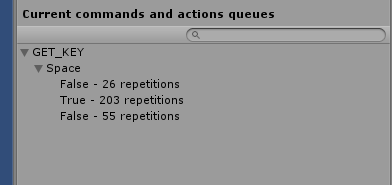
\includegraphics[width=0.7\linewidth]{storageContains.png}
	\caption{Пример работы RLE-сжатия очереди записываемых действий}
	\label{storageContains}
\end{figure}

\subsection{Система сохранения и загрузки хранилища действий}
Система сохранения и загрузки является PAC компонентом, она используется напрямую только хранилищем записанных действий. Интерфейс IATFActionStorageSaver (см. листинг \ref{iSaver}) отвечает за реализацию системы сохранения и загрузки хранилища в потенциально любой носитель информации.

Реализация интерфейса (см. листинг \ref{iSaver}) основана на работе с реестром через встроенный в стандартную библиотеку \textit{Unity} класс PlayerPrefs, обычно отвечающий за сохранение небольшой по количеству информации. Для сохранения сложных объектов эта реализация использует сериализацию в JSON объект всего хранилища либо же только одной записи, в зависимости от метода, который вызывается. Поведение реализации похоже на поведение недетерминированного автомата, по уже вышеупомянутым причинам.

\subsection{Система упаковки данных хранилища}
Для обеспечения гибкости использования алгоритмов сериализации и сжатия хранилища данных была реализована система упаковки реализующая интерфейс IAtfPacker (см. листинг \ref{iPacker}). Данная система позволяет не вмешиваясь в методы системы сохранения и загрузки менять данные для удобства сериализации и потенциальной оптимизации.

В текущей своей реализации система упаковки использует жадный алгоритм перевода данных в сериализируемую структуру классов, что призвано упростить чтение исходного кода системы сохранения и загрузки хранилища действий.

\subsection{Система интеграции в готовую кодовую базу}
Дополнительный функционал системы интеграции позволяет автоматизировать процессы интеграции ATF в сторонний проект путём поиска и замены текста исходного кода всей базы или конкретных выбранных скриптов (файлов исходного кода компонентов Unity) с помощью регулярного выражения, которое определяет использование класса Input в исходном коде. Система интеграции реализует интерфейс IAtfIntegrator (см. листинг \ref{iIntegrator}).

Данная система может функционировать в двух режимах:
\begin{itemize}
	\item Автоматический -- система сканирует всю кодовую базу стороннего проекта, находя файлы исходного кода с расширением .cs и по очереди, с помощью жадного перебора, выполняет замену имени класса Input на ATFInput, при этом не создавая новых файлов с интегрированным перехватчиком.
	\item Полуавтоматический -- система наполняется путями к файлам исходного кода вручную с помощью вспомогательного окна, а затем задействует подстановку, как и в случае с автоматическим режимом, но можно выбрать: создать дополнительный файл с суффиксом ATF, где будет уже внедрён перехватчик, или же произвести замену без создания дополнительного файла.
\end{itemize}
\chapter{Человеко-машинный интерфейс}

В рамках данной работы человеко-машинный интерфейс представлен в виде пользовательских окон управления в Unity Editor, а также в виде онлайн-ресурса посвящённого обучению и модификации описываемой работы.

\label{cha:ch_3}
При создании окон управления не были использованы ни синглтон заготовки, ни написанный DI контейнер ввиду особенностей распределения времени выполнения у \textit{Unity} -- пространство имен, взаимодействующее с классами, которые регламентируют внешний вид и поведение пользовательских окон, изолировано от других пространств, что делает невозможным использование DI и других вспомогательных структур. 

\section{Окно управления записью и проигрыванием}
Данное окно (см. рис. \ref{recorderUI}) состоит из трёх секций: указание текущей реализации проигрывателя, состояние проигрывателя и элементы управления проигрыванием и записью.

\begin{figure}[h]
	\centering
	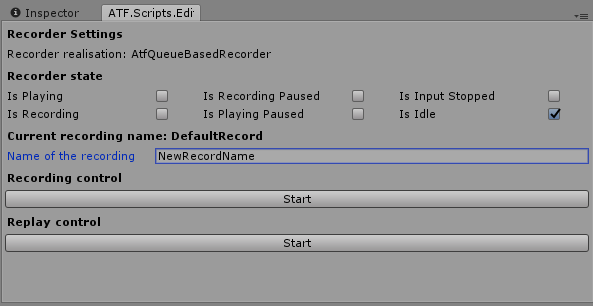
\includegraphics[width=0.7\linewidth]{recorder.PNG}
	\caption{Editor UI для проигрывателя}
	\label{recorderUI}
\end{figure}

В процесс управления записью входит:
\begin{itemize}
	\item
	просмотр текущего состояния проигрывателя по чекбоксам состояния на рис.\ref{recorderUI};
	\item
	определение имени записи, которую нужно проиграть или под которое нужно записать поток действий;
	\item
	непосредственно сами кнопки управления записью -- Start, Stop, Play, Continue;
	\item
	аналогичные кнопки управления проигрыванием -- Start, Stop, Play, Continue.
\end{itemize}
Для того чтобы проиграть выбранную запись, необходимо сначала вписать нужное имя в поле \textit{Name of the recording} или же просто щёлкнуть правой кнопкой мыши по записи в активной зоне окна управления хранилищем.

Также, была создана функция остановки ввода. Для этого необходимо нажать комбинацию клавиш ``Ctrl+I''. Мотивация к созданию функционала по остановке ввода, была в необходимости, не используя мышку, в полной мере пользоваться ATF. Существует множество приложений визуализации и игр, разработанных на платформе \textit{Unity}, которые используют мышку во время исполнения. Без возможности останавливать ввод, было бы невозможно использовать любые окна управления ATF, оставляя при этом неизменным состояние приложения.

В дополнение к возможностям управления без мышки были добавлены новые комбинации клавиш (см. рис. \ref{shortcuts}).

\begin{figure}[h]
	\centering
	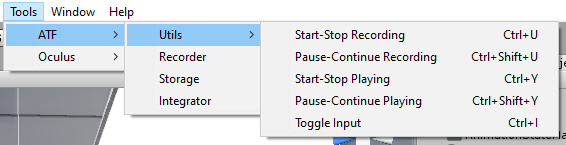
\includegraphics[width=\linewidth]{shortcuts.png}
	\caption{Комбинации клавиш управления окном записи}
	\label{shortcuts}
\end{figure}

Данные комбинации работают также как переключатели света. Другими словами, первое нажатие активирует функцию, второе -- выключает её.
\begin{itemize}
	\item ``Ctrl+U'' -- Включение или выключение записи.
	\item ``Ctrl+Shift+U'' -- Пауза или продолжение записи.
	\item ``Ctrl+Y'' -- Включение или выключение проигрывания.
	\item ``Ctrl+Shift+Y'' -- Пауза или продолжение проигрывания.
\end{itemize}

\section{Окно управления хранилища действий}
Окно управления хранилищем (см. рис. \ref{storageUI}) также состоит из трёх секций -- информация о реализации, секции управления сохранением и загрузкой, а также зоны иллюстрации текущего состояния хранилища.

\begin{figure}[h]
	\centering
	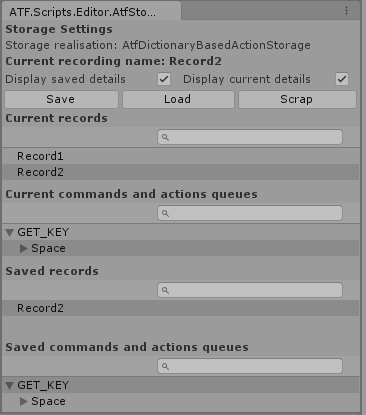
\includegraphics[width=0.7\linewidth]{storage.PNG}
	\caption{Editor UI для хранилища действий}
	\label{storageUI}
\end{figure}

В процесс управления хранилищем входит:
\begin{itemize}
	\item
	просмотр текущей записи хранилища;
	\item
	определение имени записи, которую нужно загрузить или сохранить; 
	\item
	непосредственно сами кнопки управления сохранением -- Save, Load, Scrap (удалить);
	\item
	загрузка в активную зону записей из реестра (Окна: Current records, Current commands and actions queues);
	\item экспорт и импорт записей в пассивной зоне на внешний накопитель.
\end{itemize}
Зоны иллюстрации хранилища делятся на активную и пассивную. Активная зона хранит в себе те записи, которые находятся сейчас непосредственно в оперативной памяти, пассивная же зона хранит в себе записи, которые были сохранены на внешнем накопителе или реестре.

Чтобы экспортировать всё, что находится в пассивной зоне, необходимо вписать абсолютный путь к файлу с расширением ``.json'', где и будет располагаться сохранённое хранилище. Далее необходимо нажать на кнопку \textit{Export saved storage}.

Для выполнения импорта хранилища, нужно проделать те же шаги, но путь указать к уже существующему файлу. Далее следует нажать на кнопку \textit{Import saved storage}. 

\section{Окно управления интеграцией}

Окно управления интеграцией состоит из трёх секций и работает в двух режимах интеграции и в двух режимах выбора путей. Первая секция -- информация об используемой реализации, вторая -- секция добавления и удаления путей к файлам исходного кода и третья -- секция с отображением выбранных файлов и кнопками управления.

Находясь в первом режиме выбора путей (см. рис. \ref{integratorUI}), пользователь вводит пути к файлам исходного кода, в которые следует интегрировать ATF, вручную. Вводимый путь является относительным и его корень лежит в папке Assets, в директории проекта. 

\begin{figure}[h]
	\centering
	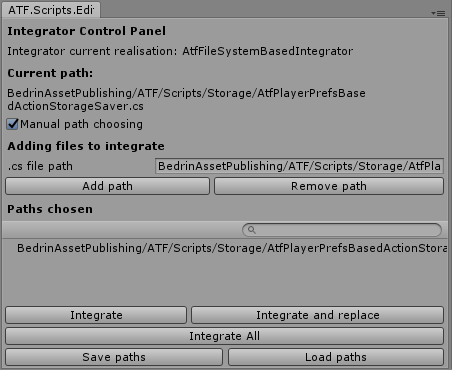
\includegraphics[width=0.7\linewidth]{integrator_manual.PNG}
	\caption{Editor UI для управления интеграцией в ручном режиме}
	\label{integratorUI}
\end{figure}

Второй режим выбора путей (см. рис. \ref{integratorUIAutomatic}) позволяет упростить и ускорить сбор путей к файлам исходного кода. Для этого нужно отключить чекбокс \textit{Manual path choosing}. После его отключения, файлы исходного кода можно выделять мышкой во вкладке Project в Unity Editor. Все выбранные файлы автоматически попадают в очередь на интеграцию.

\begin{figure}[H]
	\centering
	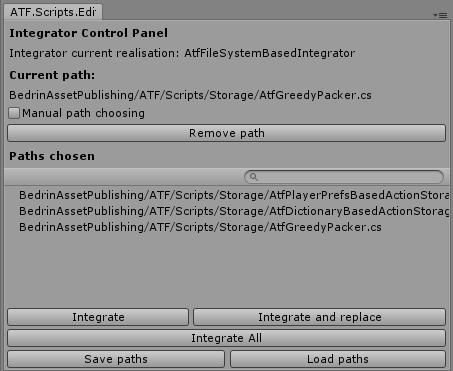
\includegraphics[width=0.7\linewidth]{integrator_automatic.PNG}
	\caption{Editor UI для управления интеграцией в автоматическом режиме}
	\label{integratorUIAutomatic}
\end{figure}

Удаление путей в обоих режима происходит одинаково: выделение пути в списке и нажатие на кнопку \textit{Remove path}. Стоит заметить, что, если не убрать полностью выделение во вкладке Project, курсор в виде текущего выбранного пути, отображаемого в секции \textit{Current path}, будет обращён на последний выделенный путь, из-за чего при невнимательном управлении можно случайно удалить не те пути, что были выбраны в списке.

Так как система интеграции поддерживает два режима работы: автоматический и полуавтоматический, при проектировании данного окна было решено выделить отдельные кнопки для обоих режимов:
\begin{itemize}
	\item
	Кнопки \textit{Integrate} и \textit{Integrate and replace} отвечают за полуавтоматический режим и воздействуют на представленные в третьей секции конкретные файлы исходного кода.
	\item
	Кнопка \textit{Integrate All} отвечает за использование автоматического режима.
\end{itemize}

Кнопки \textit{Save paths} и \textit{Load paths} отвечают за сохранение и загрузку представленных в третьей секции файлов исходного кода. Для облегчения работы с файлами, вместо конкретных файлов во второй секции было решено использовать пути файлов.

\section{Онлайн-документация и способ доступа}
Для лучшего понимания функционала разработанной группы ассетов была создана онлайн-документация \cite{atf_docs}. Данный ресурс содержит в себе учебный материал не только для обучения пользованием ассетами, но и информацию о каждом интерфейсе основной системы и учебный материал, где рассказывается о том, как можно модифицировать разработанные ассеты, а также создавать новые. 

В качестве платформы для создания онлайн-документации было решено использовать ReadTheDocs.org (RTD) с генератором документации Sphinx (см. рис. \ref{online_docs}). Критерием к выбору платформы и генератора служила возможность бесплатного хостинга ресурса с адекватным на мнение автора именем хоста, лёгкость языка шаблонизатора у генератора, а также высокий уровень репутации ресурса.

Процесс развёртывания данной онлайн-документации на платформе RTD заключается всего в двух шагах: инициализация в сервисе хостинга github-репозитория с исходным кодом статей на языке ReST и запрос на автоматическую сборку и развёртывание онлайн-документации.

\begin{figure}[H]
	\centering
	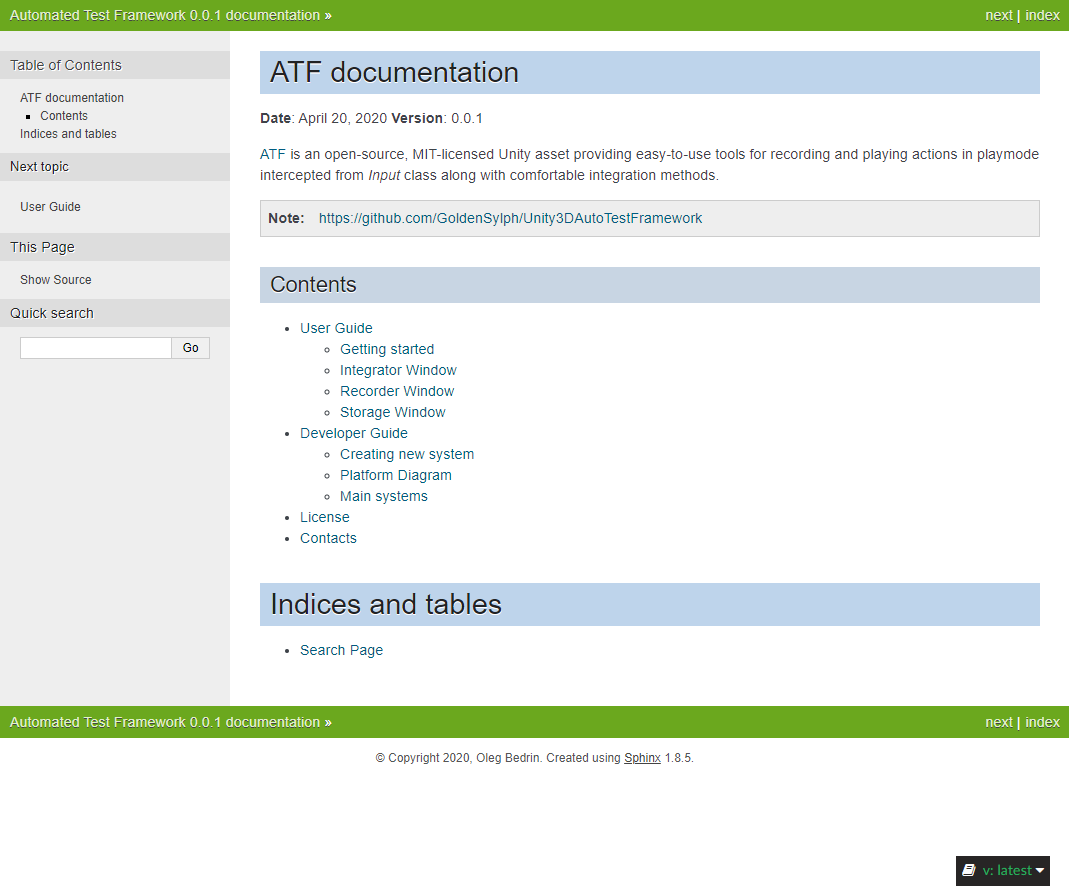
\includegraphics[width=\linewidth]{online_docs.png}
	\caption{Главная страничка онлайн-документации}
	\label{online_docs}
\end{figure}

Это было необходимо, чтобы не отпугнуть потенциального контрибьютора от изучения документации. Возможности контрибьютинга (совместной разработки с публикой) обусловлены тем, что лицензия результатов данной разработки создана на основе MIT.

В дополнение к созданной онлайн-документации, была добавлена возможность быстрого поиска по статьям, представленным в ней. В качестве языка шаблонов был использован reStructuredText -- облегчённый язык разметки схожий по синтаксису с языком Markdown, однако позволяющий автоматически генерировать файлы PDF, HTML, ODT, LaTeX, а также формат презентаций S5.

Так как разработанная группа ассетов распространяется по лицензии MIT, доступ к исходному коду открыт и доступен на сайте GitHub.com \cite{git}.

В руководство для пользователей (разработчиков проекта, в который ATF был интегрирован) входит множество инструкций по использованию ATF (см. рис. \ref{user_online_docs}). 

Первая инструкция посвящена интеграции ATF в новый пустой проект. Там иллюстрируюется способ доступа к свежему пакету с ATF, а также объясняется как подготовить сцену и где найти управляющие окна. Вторая инструкция демонстрирует интеграцию в существующий проект и аспекты использования статического или объектного доступа к перехатчику. Третья и четвертая инструкции иллюстрирует работу всех режимов перехватчика и окна записи соответственно. Здесь объясняется то, как можно использовать механизм остановки ввода, не нарушая состояния приложения во время исполнения. Пятая инструкция посвящена функционалу манипулирования хранилищем действий, описывая его зоны для просмотра содержания записи и функции его импорта и экспорта. Заключительная шестая инструкция объясняет как пользоваться комбинациями клавиш для управления записью.

\begin{figure}[H]
	\centering
	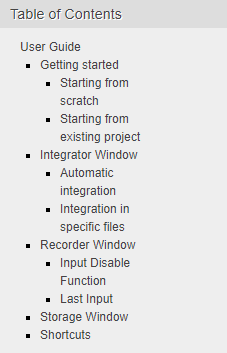
\includegraphics[width=0.3\linewidth]{user_guide.PNG}
	\caption{Содержание руководства для пользователей}
	\label{user_online_docs}
\end{figure}

В руководство для контрибьюторов (см. рис. \ref{dev_online_docs}) входят обзорные статьи посвященные принципам построения кодовой базы ATF.

Первая статья посвящена созданию новой системы, которая бы автоматически инициализировалась на сцене, сразу же после инъекции зависимостей. Вторая статья посвящена обзору платформы ATF и тому, как организовано взаимодействие со стандартными системами \textit{Unity}. Заключительная статья содержит описания всех интерфейсов основных систем ATF, включая комментарии по хранению данных и модификации.

\begin{figure}[H]
	\centering
	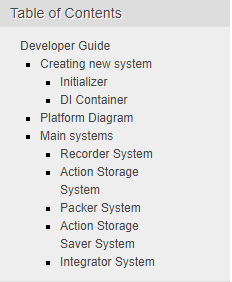
\includegraphics[width=0.3\linewidth]{dev_guide.PNG}
	\caption{Содержание руководства для контрибьюторов}
	\label{dev_online_docs}
\end{figure}


\backmatter %% Здесь заканчивается нумерованная часть документа и начинаются ссылки и
            %% заключение

\Conclusion
Согласно цели и задачам поставленным в начале данной выпускной квалификационной работы были получены результаты, которые позволяют не только разрешить указанную проблему формального исполнителя для регрессионного тестирования, но и в дополнение применить эффективную \cite{open_source} модель дальнейшего развития проекта в качестве open-source ПО.

В процессе исследования популярности выбранного способа запрашивания ввода на платформе \textit{Unity} были созданы несколько версий spider-программ, однако предпочтения были отданы одной, которая в своём ядре разделяет процесс сбора данных с помощью параллельных вычислений. Также, в качестве приёма доказательства поставленной гипотезы была адаптирована под логическую функцию тождественности цепочка статистических выводов, что позволило успешно завершить исследование и приступить к проектированию.

Краткий анализ класса совместимых приложений позволил выделить основные приёмы разработки, которые были использованы для аналогов с других платформ. Были определены конкретные шаблоны проектирования и стратегические направления в развитии архитектуры группы ассетов имеющие фундаментальные основания в объектно-ориентированном программировании.

Реализация системы управления зависимостями и автоматический инициализации перехватчика ввода позволило очистить исходный код основных систем от сквозного кода благодаря использованию приёмов программной рефлексии (обращению к единицам компиляции как к классам и объектам) и возможностям языка программирования CSharp создавать атрибуты классов (аннотативные сущности несущие вспомогательную информацию).

Главным выводом по факту создания основных систем группы ассетов, является то, что в большинстве своём исходный код подчиняется основным принципам проектирования SOLID характерным для enterprise-проектов в объектно-ориентированном программировании. Это позволяет производить масштабирование функционала системы используя всего два действия: создание .cs файла и аннотирование специальными атрибутами декларацию и зависимости класса добавляемой системы. Дальше, при переходе Unity Editor в Play Mode разработанная группа ассетов сама настроит новый функционал.

Благодаря выбранной архитектуре и построении зависимостей над абстрактными сущностями (интерфейсами, абстрактными классами и т.д.), все записи действий могут быть экспортированы и импортированы согласно двум основным системам: системе упаковки и системе сохранения и загрузки хранилища действий. Каждая из этих систем использует сигнатуры методов интерфейсов, поэтому создание и модификация этих систем не приведёт к лавинному эффекту с правками кода.

Реализация пользовательских окон управления данной группой ассетов для Unity Editor позволило быстро взаимодействовать с перехватом и записью действий без создания дополнительной кодовой базы, как если бы результаты данной работы были лишь представлены в виде Application Programmable Interface (API).

Говоря о полноте решений поставленных задач, конечно нельзя не заметить, что хоть и класс Input является самым распространённым среди других способов запрашивания ввода, огромная часть приложений использует и другие способы, а также их комбинации, в зависимости от целевой платформы сборки. Из этого следует, что дальнейший вектор развития данной работы указывает на охват большего количества способов запрашивания ввода. 

В дополнение, развитие платформы \textit{Unity} тоже не стоит на месте, способ Input System описанный в начале второй главы активно развивается и постепенно станет доминировать при переходе с объектно-ориентированного подхода к построению Unity-приложений к ориентированному на данные. Данный прогноз исходит из того, что если сейчас построить Unity-приложение с помощью уже существующих ориентированных на данные приёмов, то использование других способов запрашивания ввода станет технически невозможным.

Результат данной работы рекомендуется использовать в проектах с длинным временем прохождения и с линейным или частично линейным потоком действий. Также, благодаря активному развитию, следует осторожно использовать данную группу ассетов, так как ни один разработчик не застрахован от совершения алгоритмических ошибок.

\nocite{*}
%\bibliographystyle{gost780u}
%\bibliography{0-main}
\begin{thebibliography}{9} 
	
	\bibitem{selenium} Vila E., Novakova G., Todorova D. Automation Testing Framework for Web Applications with Selenium WebDriver: Opportunities and Threats // Proceedings of the International Conference on Advances in Image Processing (ICAIP 2017). 2017. P. 144-150.
	
	\bibitem{rpc_testing} Sinaga A. M., Adi Wibowo P., Silalahi A., Yolanda N. Performance of Automation Testing Tools for Android Applications // 10th International Conference on Information Technology and Electrical Engineering (ICITEE). 2018. P. 534-539.
	
	\bibitem{appium_opencv} Mozgovoy M., Pyshkin E. Unity Application Testing Automation with Appium and Image Recognition // In: Itsykson V., Scedrov A., Zakharov V. (eds) Tools and Methods of Program Analysis. TMPA 2017. Communications in Computer and Information Science. 2017. №779. P. 139--150.
	
	\bibitem{wimp} Andries van Dam Post-WIMP user interfaces // Commun. ACM. 1997. №2. P. 63–67.
	
	\bibitem{habr} Лучший игровой движок по версии пользователей хабра // Хабр URL: https://habr.com/ru/post/307952/ (дата обращения: Апрель 11, 2020).
	
	\bibitem{disser} Кугуракова В.В МАТЕМАТИЧЕСКОЕ И ПРОГРАММНОЕ ОБЕСПЕЧЕНИЕ МНОГОПОЛЬЗОВАТЕЛЬСКИХ ТРЕНАЖЕРОВ С ПОГРУЖЕНИЕМ В ИММЕРСИВНЫЕ ВИРТУАЛЬНЫЕ СРЕДЫ: дис. ... канд. тех. наук: 05.13.11. Казань, 2019. 187 с.
	
	\bibitem{vr-simulators} Kugurakova V.V. Automated approach to creating multi-user simulators in virtual reality // CEUR Workshop Proceedings. 2018. №2260. P. 313-320.  
	
	\bibitem{visual-editor} Kugurakova V.V., Abramov V.D., Abramsky M.M., Monks N., Maslaviev A. Visual editor of scenarios for virtual laboratories // DeSE 2017, Developments in the design of electronic systems.. Paris: Conference Publication Services (CPS), 2017. P. 242-247.
	
	%%% Вступление остортировано
	
	\bibitem{unity_input_systems} Unity -- Manual: Input // Unity Manual URL: https://docs.unity3d.com/Manual/Input.html (дата обращения: Апрель 12, 2020).
	
	\bibitem{solid} Мартин Р.С., Ньюкирк Д.В., Косс Р.С. Быстрая (гибкая) разработка программ на Java и C++: принципы, шаблоны, практика. М.: Издательский дом ``Вильямс'', 2001. 752 с.

	\bibitem{dry} Haoyu W., Haili Z. Basic Design Principles in Software Engineering // Fourth International Conference on Computational and Information Sciences. Chongqing: IEEE Computer Society, 2012. P. 1251-1254.
	
	\bibitem{razor} Blumer A., Ehrenfeucht A., Hasler D., Warmuth M.K. Occam's Razor // Information Processing Letters 24. 1987. №6. P. 377-380.
	
	\bibitem{dots} High-performance multithreaded stack of unity information-oriented technologies // unity.com URL: https://unity.com/ru/dots (дата обращения: Июль 19, 2019).
	
	\bibitem{ecs} Unity Foundation -- Introduction to ECS // unity3d.com URL: https://unity3d.com/ru/learn/tutorials/topics/scripting/introduction-ecs (дата обращения: Июль 19, 2019).
	
	\bibitem{interceptor} Schmidt D., Stal M., Rohnert H., Buschmann F. Pattern-Oriented Software Architecture // Patterns for Concurrent and Networked Objects. 2001. №2. P. 109-140.
	
	\bibitem{broker} Architectural pattern ``Broker'' // cs.uno.edu URL: http://cs.uno.edu/~jaime/Courses/4350/broker.ppt (дата обращения: Июль 19, 2019).
	
	\bibitem{pac} Coutaz J. PAC: AN OBJECT ORIENTED MODEL FOR IMPLEMENTING USER INTERFACES // ACM SIGCHI Bulletin. 1987. №19. P. 37-41.
	
	\bibitem{jsr} JSR 299: Contexts and Dependency Injection for the JavaTM EE platform // jcp.org URL: https://jcp.org/en/jsr/detail?id=299 (дата обращения: Июль 19, 2019).
	
	\bibitem{oreilly} Брюс П., Брюс Э. Практическая статистика для специалистов Data Science. СПб.: БХВ-Петербург, 2018. 304 с.
	
	
\end{thebibliography}
\appendix   % Тут идут приложения
\chapter{Листинги}
\section{Исходный код класса обработки веб-страниц проектов с сайта GitHub.com}
\begin{lstlisting}[caption={Исходный код класса обработки веб-страниц проектов с сайта GitHub.com},label=spider]

# -*- coding: utf-8 -*-
import scrapy
import requests
import json
import base64
import re
import time
import pandas as pd
class GithubSpiderSpider(scrapy.Spider):

	name = 'github-spider'
	main_data = pd.DataFrame(columns=['repo_name', 'method_invocations'])
	file_name = 'main_data_most_forks.csv'
	config = False
	recently_updated_url = 
	'https://github.com/search?o=desc&p={}
		&q=unity+language%3AC%23&s=updated&type=Repositories'
	most_stars_url = 
	'https://github.com/search?o=desc&p={}
		&q=unity+language%3AC%23&s=stars&type=Repositories'
	most_forks_url = 
	'https://github.com/search?o=desc&p={}
		&q=unity+language%3AC%23&s=forks&type=Repositories'
	best_match_url = 
	'https://github.com/search?p={}
		&q=language%3Acsharp+unity&type=Repositories'

	def start_requests(self):
		urls = [self.most_forks_url.format(i + 1) for i in range(101)]
		for url in urls:
			yield scrapy.Request(url=url, callback=self.parse)
	
	def auth_data(self):
		if self.config:
			return (self.config['login'], self.config['password'])
		with open('github_config.json', 'r', encoding='utf-8') as github_file:
			self.config = json.load(github_file)
			return (self.config['login'], self.config['password'])
		
	def get(self, url):
		result = requests.get(url, auth=self.auth_data())
		if result.status_code == 403:
			header_name = 'X-RateLimit-Reset'
			if header_name in result.headers:
				reset_time = float(result.headers[header_name])
				sleep_time = reset_time - time.time()
				if sleep_time < 0:
					self.logger.info('Sleep time is negative, adjusting to 1...')
					sleep_time = 1
				self.logger.info('Exceeded rate limit. Waiting for: {}'.format(sleep_time))
				time.sleep(sleep_time)
				result = requests.get(url, auth=auth_data)
			else:
				return False
				self.logger.info('{}, status: {}'.format(result.headers, result.status_code))
		return result
	
	def get_json(self, response):
		try:
			return response.json()
		except:
			self.logger.info(traceback.format_exc())
			return False
	
	def closed(self, reason):
		self.logger.info('Done. Specified reason: {}'.format(str(reason)))
	
	def parse(self, response):
		repo_names = [r[1:] for r in response.xpath('//div[@class="f4 text-normal"]/a/@href').extract()]
		for repo_name in repo_names:
		self.logger.info('Working with repo: {}'.format(repo_name))
		code_search_url = 'https://api.github.com/search/code?
			q=Input+in:file+language:csharp+repo:{}'
			.format(repo_name)
		code_response = self.get(code_search_url)
		if not code_response:
			self.logger.info('something wrong with header, continue...')
			continue
		code_data = self.get_json(code_response)
		if not code_data:
			continue
		method_invokations_count = 0
		code_urls = [code_item['url'] for code_item in code_data['items']]
		for code_url in code_urls:
			self.logger.info('Source url: {}'.format(code_url))
			source_details_response = self.get(code_url)
			if not source_details_response:
				self.logger.info('something wrong with header in source details response, continue...')
				continue
			source_details_data = self.get_json(source_details_response)
			if not source_details_data:
				continue
			if 'message' in source_details_data:
				self.logger.info(source_details_data['message'])
				continue
			try:
				source = 
				base64.b64decode(source_details_data['content']
					.encode('utf-8')).decode('utf-8')
			except:
				self.logger.info(traceback.format_exc())
				continue
			method_invokations_count_in_source = 
				len(re.findall(r'[(\[(\s,=\+\-\*/\?&|]Input\.', source))
			method_invokations_count += method_invokations_count_in_source
		new_data = pd.DataFrame({'repo_name': repo_name, 'method_invocations': method_invokations_count}, index=[0])
		self.main_data = self.main_data.append(new_data, ignore_index=True)
		self.logger.info('Data gathered:\n{}'.format(new_data))
		self.main_data.to_csv(self.file_name)
\end{lstlisting}
\newpage
\section{Утилита для сбора собранных spider-программой данных воедино}
\begin{lstlisting}[caption={Утилита для сбора собранных spider-программой данных воедино},label=form_main_data]
import pandas as pd
import seaborn as sns
import matplotlib.pyplot as plt
sns.set(style="white", context="talk")
whole_data = pd.DataFrame(columns=['repo_name', 'method_invocations', 'filter'])
metadata = [('main_data_best_match.csv', 'best_match'),
('main_data_most_stars.csv', 'most_stars'),
('main_data_most_forks.csv', 'most_forks'),
('main_data_recently_updated.csv', 'recently_updated')]
for data in metadata:
	new_data = pd.read_csv(data[0], index_col=0)
	new_data['filter'] = data[1]
	whole_data = whole_data.append(new_data, ignore_index=True)
whole_data['filter'] = whole_data['filter'] + whole_data.duplicated(subset='repo_name').apply(str)
print(whole_data)
whole_data.to_csv('main_data.csv')
sns.scatterplot(x=whole_data.index, y='method_invocations', data=whole_data, hue='filter')
plt.show()
plt.clf()
\end{lstlisting}
\newpage
\section{Утилита для проведения бутстрапа и параллельных расчётов границ интервала среднего}
\begin{lstlisting}[caption={Утилита для проведения бутстрапа и параллельных расчётов границ интервала среднего},label=bootstrap_experiment]

import math as m
import pandas as pd
import multiprocessing as mp
import seaborn as sns
import matplotlib.pyplot as plt
import matplotlib

def stat(x):
return round(x.mean(), 3)

if __name__ == '__main__':

	whole_data = pd.read_csv('main_data.csv')
	
	R = 99509
	n = len(whole_data)
	confidence = 90
	specific_data = whole_data['method_invocations']
	
	process_count = mp.cpu_count()
	chunk_size = 1000
	print('Processes: {}, chunksize: {}'.format(process_count, chunk_size))
	
	with mp.Pool(process_count) as pool:
		boot_data =
		pd.Series(pool.map(stat, 
			[specific_data.sample(n, replace=True) for i in range(R)], 
				chunksize=chunk_size))
	
	boot_data_len = len(boot_data)
	cut_percent = m.ceil((1 - confidence / 100) / 2)
	cut = round(boot_data_len * cut_percent / 100)
	middle_cuts = [cut, boot_data_len - cut]
	tail_cut = boot_data_len - cut
	print('boot_data_len: {}, cut_percent: {}, cut: {}, middle_cuts: {}, tail_cut: {}'.format(boot_data_len, cut_percent, cut, middle_cuts, tail_cut))
	head = boot_data[:cut]
	middle = boot_data[middle_cuts[0]:middle_cuts[1]]
	tail = boot_data[tail_cut:]
	main_data = pd.DataFrame(columns=['stat', 'kind'])
	main_data = main_data.append(pd.DataFrame({'stat': head, 'kind': 'head'}), ignore_index=True)
	main_data = main_data.append(pd.DataFrame({'stat': middle, 'kind': 'interval'}), ignore_index=True)
	main_data = main_data.append(pd.DataFrame({'stat': tail, 'kind': 'tail'}), ignore_index=True)
	sns.jointplot(x=main_data.index, y=main_data['stat'], kind='hex')
	plt.axhline(y=main_data.at[cut, 'stat'], color='r')
	plt.axhline(y=main_data.at[tail_cut, 'stat'], color='r')
	plt.text(cut, main_data.at[cut, 'stat'] + 0.01, 'L: {}'.format(main_data.at[cut, 'stat']), fontsize=12)
	plt.text(cut, main_data.at[tail_cut, 'stat'] + 0.01, 'U: {}'.format(main_data.at[tail_cut, 'stat']), fontsize=12)
	plot_backend = matplotlib.get_backend()
	mng = plt.get_current_fig_manager()
	if plot_backend == 'TkAgg':
		mng.resize(*mng.window.maxsize())
	elif plot_backend == 'wxAgg':
		mng.frame.Maximize(True)
	elif plot_backend == 'Qt4Agg':
		mng.window.showMaximized()
	plt.savefig('experiment.png')
	plt.show()


\end{lstlisting}
\newpage
\section{Интерфейс модуля загрузчика хранилища записей}
\begin{lstlisting}[caption={Интерфейс модуля загрузчика хранилища записей},label=iSaver]
public interface IATFActionStorageSaver : IATFInitializable
{
	void SaveRecord();
	void LoadRecord();
	void ScrapRecord();
	
	IEnumerable GetActions();
	void SetActions(IEnumerable actionEnumerable);
	List<TreeViewItem> GetSavedNames();
	List<TreeViewItem> GetSavedRecordDetails(string recordName);
}
\end{lstlisting}
\newpage
\section{Интерфейс модуля хранилища записей}
\begin{lstlisting}[caption={Интерфейс модуля хранилища записей},label=iStorage]
public interface IATFActionStorage : IATFInitializable
{
	object GetPartOfRecord(FakeInput kind, object fakeInputParameter);
	void Enqueue(string recordName, FakeInput kind, object fakeInputParameter, AtfAction atfAction);
	AtfAction Dequeue(string recordName, FakeInput kind, object fakeInputParameter);
	AtfAction Peek(string recordName, FakeInput kind, object fakeInputParameter);
	bool PrepareToPlayRecord(string recordName);
	void ClearPlayStorage();
	void SaveStorage();
	void LoadStorage();
	void ScrapSavedStorage();
	List<TreeViewItem> GetSavedRecordNames();
	List<TreeViewItem> GetCurrentRecordNames();
	List<TreeViewItem> GetCurrentActions(string recordName);
	List<TreeViewItem> GetSavedActions(string recordName);
}
\end{lstlisting}
\newpage
\section{Бизнес-логика MonoSingleton<T>}
\begin{lstlisting}[caption={Бизнес-логика MonoSingleton<T>},label=monoSingleton]
public class MonoSingleton<T> : MonoBehaviour where T : MonoBehaviour
{
	private static T s_Instance;
	private static bool s_IsDestroyed;
	public static T Instance
	{
	get
	{
	if (s_IsDestroyed)
	return null;
	if (s_Instance == null)
	{
	s_Instance = FindObjectOfType(typeof(T)) as T;
	
	if (s_Instance == null)
	{
	var gameObject = new GameObject(typeof(T).Name); 
	DontDestroyOnLoad(gameObject);
	s_Instance = gameObject.AddComponent(typeof(T)) as T;
	}
}
return s_Instance;
...
}
\end{lstlisting}
\newpage
\section{Метод инъекции зависимостей в экземпляр класса типа}
\begin{lstlisting}[caption={Метод инъекции зависимостей в экземпляр класса типа},label=injectType]
public static void InjectType(Type t)
{
	if (!ContainsAnyAttributeOfType(
	t.GetCustomAttributes(false), typeof(InjectableAttribute))) return;
		foreach (var fi in t.GetFields())
	{
	...
	if (temp.ComponentType == null && isScenePathEmpty) temp.ComponentType = fi.FieldType;
	...
	if (!isScenePathEmpty)
	{
		var hierarchyAndComponent = GetHierarchyPathAndComponentName(temp.ScenePath);
		if (!hierarchyAndComponent.Valid)
		{
			... continue;
		} 
		gameObjectContainingObjectToInject = GameObject.Find(hierarchyAndComponent.Result[0]);
		if (!gameObjectContainingObjectToInject)
		{
			... continue;
		}
		objectToInject = gameObjectContainingObjectToInject
		.GetComponent(hierarchyAndComponent.Result[1]);
	}
	else
	{
		objectToInject = FindObjectOfType(temp.ComponentType);
		if (objectToInject)
		{
			gameObjectContainingObjectToInject = GameObject.Find(objectToInject.name);
		}
		if (!gameObjectContainingObjectToInject && !temp.LookInScene)
		{
			objectToInject = Activator.CreateInstance(temp.ComponentType) as UnityEngine.Object;
			if (!objectToInject)
			{
				... continue;
			} ...
		}
	}
	if (!gameObjectContainingObjectToInject && objectToInject == null && temp.LookInScene)
	{
	... continue;
	}
	...
	dynamic typeToWhichInjected = FindObjectOfType(t.GetTypeInfo());
	if (typeToWhichInjected == null)
	{
	... continue;
	}
	fi.SetValue(typeToWhichInjected, objectToInject);
	...
}
\end{lstlisting}
\newpage
\section{Бизнес-логика базовой системы интеграции}
\begin{lstlisting}[caption={Бизнес-логика базовой системы интеграции},label=initializer]
public class ATFInitializer : MonoBehaviour
{
	private void Awake()
	{
		IATFInitializable[] ALL_SYSTEMS = {
			ATFQueueBasedRecorder.Instance, 
			ATFDictionaryBasedActionStorage.Instance,
			ATFPlayerPrefsBasedActionStorageSaver.Instance
		};
		foreach (IATFInitializable i in ALL_SYSTEMS)
		{
			i.Initialize();
		}
		DependencyInjector.Instance.Initialize("ATF");
		DependencyInjector.Instance.Inject();
	}
}
\end{lstlisting}
\newpage
\section{Бизнес-логика системы симуляции и перехвата ввода}
\begin{lstlisting}[caption={Бизнес-логика системы симуляции и перехвата ввода},label=input]
[Injectable]
[Serializable]
[AtfSystem]
public class ATFInput : MonoSingleton<T>, IBaseInput
{
[Inject(typeof(ATFQueueBasedRecorder))]
public static readonly IATFRecorder RECORDER;
[Inject(typeof(ATFDictionaryBasedActionStorage))]
public static readonly IATFActionStorage STORAGE;
[Inject(typeof(BaseInput))]
public static readonly BaseInput BASE_INPUT;
...
private static object RealOrFakeInputOrRecord(object realInput, object fakeInput, object fip, FakeInput kind)
{ ... }
private static object GetCurrentFakeInput(FakeInput inputKind, object fip)
{
return STORAGE.GetPartOfRecord(inputKind, fip);
}
...
private static T Intercept<T>(T realInput, FakeInput fakeInputKind, object 	fakeInputParameter = null)
{
    if (fakeInputParameter == null)
    {
        fakeInputParameter = "EMPTY FAKE INPUT PARAMETER";
    }
    dynamic result = RealOrFakeInputOrRecord(realInput, fakeInputParameter, fakeInputKind);
    if (result is string)
    {
        Debug.Log(result);
    }
    return result;
}
public static bool anyKeyDown => Intercept(Input.anyKeyDown, FakeInput.ANY_KEY_DOWN, false);
...
}
\end{lstlisting}
\newpage
\section{Интерфейc модуля записи}
\begin{lstlisting}[caption={Интерфейc модуля записи},label=iRecorder]
using ATF.Scripts.Helper;
namespace ATF.Scripts.Recorder
{
    public interface IAtfRecorder : IAtfGetSetRecordName
    {
        bool IsRecording();
        bool IsPlaying();
        bool IsRecordingPaused();
        bool IsPlayPaused();
        bool IsInputStopped();
        void PlayRecord();
        void PausePlay();
        void ContinuePlay();
        void StopPlay();
        void StartRecord();
        void PauseRecord();
        void ContinueRecord();
        void StopRecord();
        void SetRecording(bool value);
        void SetPlaying(bool value);
        void SetRecordingPaused(bool value);
        void SetPlayPaused(bool value);
        void SetInputStopped(bool value);
        void Record(FakeInput kind, object input, object fakeInputParameter);
        object GetLastInput(FakeInput kind, object fakeInputParameter);
        void SetLastInput(FakeInput kind, object realInput, object fakeInputParameter); ...
\end{lstlisting}
\newpage
\section{Пользовательский модуль ввода для ATFInput}
\begin{lstlisting}[caption={Пользовательский модуль ввода для ATFInput},label=inputModule]
namespace ATF
{
	public class ATFStandaloneInputManager : StandaloneInputModule
	{
		protected override void Start()
        {
            base.Start();
            m_InputOverride = AtfInput.BASE_INPUT;
            DependencyInjector
            	.InjectType(m_InputOverride.GetType());
        }
...
\end{lstlisting}
\newpage
\section{Интерфейс модуля интеграции в готовую кодовую базу}
\begin{lstlisting}[caption={Интерфейс модуля интеграции в готовую кодовую базу},label=iIntegrator]
using System.Collections.Generic;
using ATF.Scripts.Helper;
namespace ATF.Scripts.Integration.Interfaces
{
	public interface IAtfIntegrator : IAtfGetSetRecordName
	{
		void SetUris(IEnumerable<string> filePaths);
		void Integrate();
		void IntegrateAndReplace();
		void IntegrateAll();
		void SaveUris();
		IEnumerable<string> LoadUris();
	}
}
\end{lstlisting}
\newpage
\section{Интерфейс модуля упаковки хранилища данных}
\begin{lstlisting}[caption={Интерфейс модуля упаковки хранилища данных},label=iPacker]
using System.Collections.Generic;
using ATF.Scripts.Storage.Utils;
using UnityEngine;
namespace ATF.Scripts.Storage.Interfaces
{
	public interface IAtfPacker
	{
		List<Record> Pack(Dictionary<string, Dictionary<FakeInput, Dictionary<object, AtfActionRleQueue>>> input);
		Dictionary<string, Dictionary<FakeInput, Dictionary<object, AtfActionRleQueue>>> Unpack(Slot slot);
		string ValidatePacked(List<Record> packed);
	}
}
\end{lstlisting}
\newpage
\section{Пример изменения тела метода и параметра класса Input в классе-арбитре ATFInput}
\begin{lstlisting}[caption={Пример изменения тела метода и параметра класса Input в классе-арбитре ATFInput},label=atf_methods_refactor_example]
//CSharp 7.0
public static bool simulateMouseWithTouches
{
	get => Intercept(Input.simulateMouseWithTouches, 	FakeInput.SIMULATE_MOUSE_WITH_TOUCHES, "Simulate mouse with touches");
	set => Input.simulateMouseWithTouches = value;
}
//CSharp 6.0
public static bool simulateMouseWithTouches
{
	get { return Intercept(Input.simulateMouseWithTouches, 	FakeInput.SIMULATE_MOUSE_WITH_TOUCHES, "Simulate mouse with touches"); }
	set { Input.simulateMouseWithTouches = value; }
}
...
//CSharp 7.0
public static bool GetMouseButton(int button) => Intercept(Input.GetMouseButton(button), FakeInput.GET_MOUSE_BUTTON, button);

//CSharp 6.0
public static bool GetMouseButton(int button)
{
	return Intercept(Input.GetMouseButton(button), FakeInput.GET_MOUSE_BUTTON, button); ...
\end{lstlisting}
\chapter{Алгоритмы}
\section{Работа инициализатора решения}
\begin{algorithm}
	\caption{Работа инициализатора решения}\label{alg:initializer}
	\begin{algorithmic}
		\State $allSystems \gets IAtfInitializable[3]$
		\State $allSystems[0] \gets Recorder.Instance$
		\State $allSystems[1] \gets Storage.Instance$
		\State $allSystems[2] \gets Saver.Instance$
		\ForAll{system in allSystems} \State{system.Initialize()} \EndFor
		\State $DependencyInjector.InjectIntoNamespace('ATF')$
	\end{algorithmic}
\end{algorithm}
\newpage
\section{Перехват и симуляция для Input.anyKeyDown}
\begin{algorithm}
	\caption{Перехват и симуляция для Input.anyKeyDown}\label{alg:input}
	\begin{algorithmic}
		\Procedure{AtfInput.anyKeyDown}{}
		\State \textbf{return} Intercept(Input.anyKeyDown, 
		\State GetCurrentFakeInput())
		\EndProcedure
		\Procedure{Intercept}{RealInput, FakeInput}
		\State \textbf{dynamic} result := RealOrFakeInputOrRecord(RealInput, FakeInput)
		\If{result is string}
		\State \textbf{throw} new Exception(\$"Deserialization failed: \{result\}")
		\EndIf
		\State \textbf{return} result
		\EndProcedure
		\Procedure{RealOrFakeInputOrRecord}{RealInput, FakeInput}
		\If{is Recording}
		\State Recorder.Record(RealInput)
		\State \textbf{return} RealInput
		\ElsIf{is Playing}
		\State \textbf{return} FakeInput
		\Else
		\State \textbf{return} RealInput
		\EndIf
		\EndProcedure
	\end{algorithmic}
\end{algorithm}

\end{document}
